% rutowski.tex

\section{Radiating argon shock layer with thermochemical nonequilibrium}
\label{sec:rutowski}
\index{radiation transport model!example of use}
\index{finite-rate chemistry!example of use}
\index{energy exchange!example of use}
\index{gas model!two temperature!example of use}
%

\subsection{Experiment description}

\begin{figure}[b!]
 \centering
 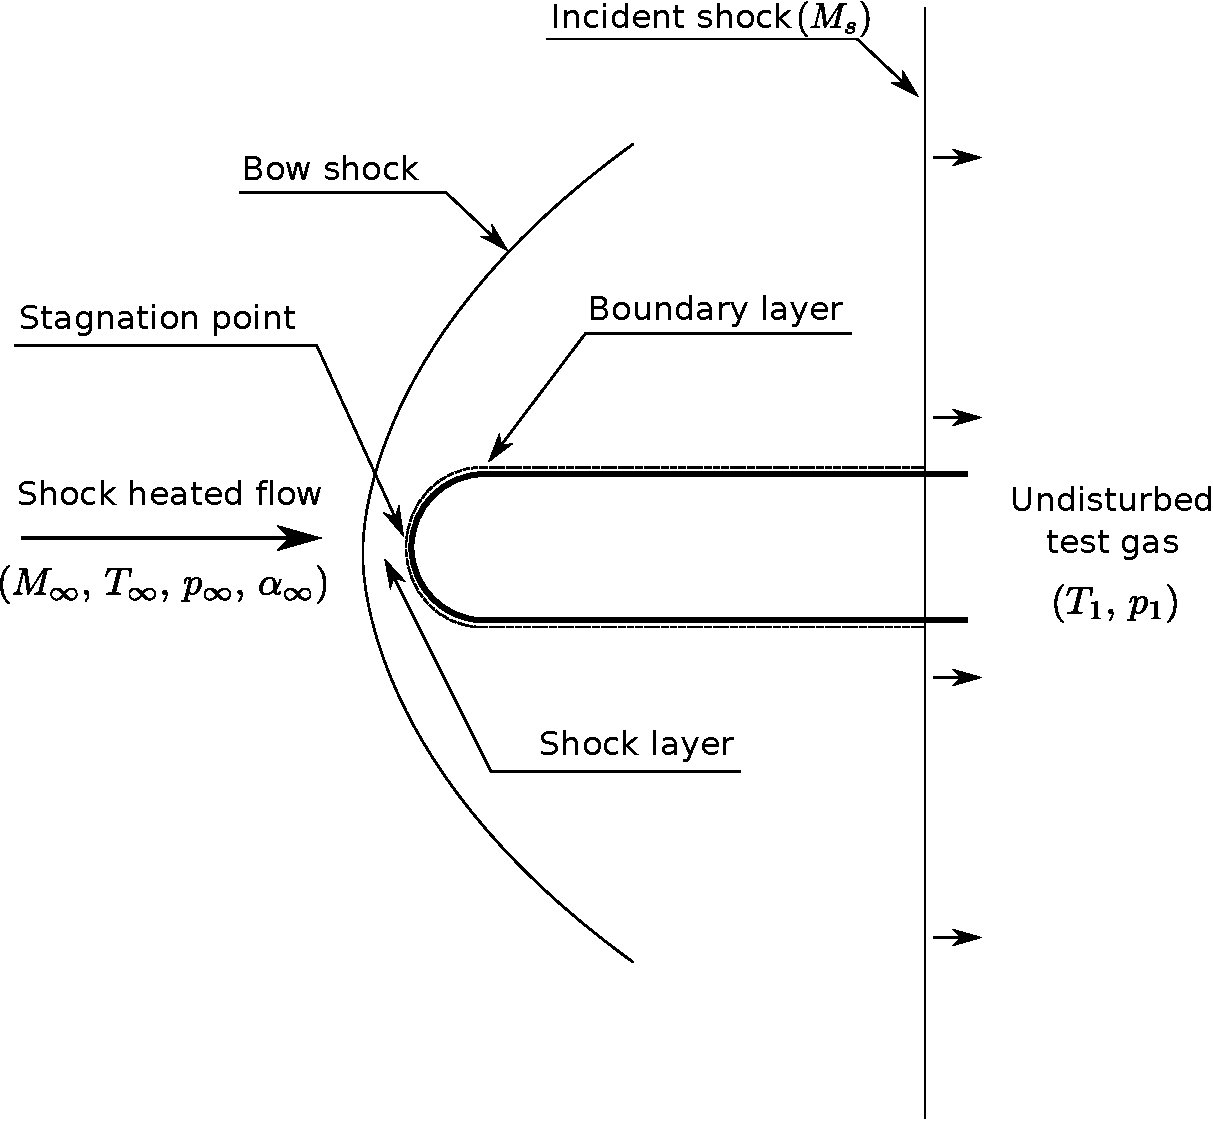
\includegraphics[scale=0.5]{../2D/Rutowski-hemisphere/figures/schematic.pdf}
 \caption{Schematic diagram of hemispherical model immersed in shock heat flow (adapted from Rutowski \textit{et al.}~\cite{RB64}).}
  \label{fig:rutowskiSchematic}
\end{figure}

Rutowski \textit{et al.}~\cite{RB64} measured the total and radiative heat fluxes at the stagnation point of a 1\,inch diameter hemisphere immersed in a freestream flow of shock heated argon.
A schematic of the experimental setup is depicted in Figure~\ref{fig:rutowskiSchematic}.
The hemispherical model was placed in the test section of a 3 inch diameter stainless steel shock tube at the Lockheed Research Laboratories~\cite{MBR+62}.  
Incident shock waves with velocities up to 4.3\,km/s ($M_s = 13.2$) were driven through the argon test gas at an initial pressure of 10\,Torr.
Total heat transfer at the stagnation point was measured with a surface mounted calorimetric gauge, in which a thin strip of polished platinum is exposed to the flow and the heat transfer determined from change in resistivity.
Radiative heat transfer was measured with a similar gauge mounted behind a sapphire window that allowed transmission in the wavelength range $180 \leq \lambda \leq 6000$\,nm.
The platinum strip was determined to have a weighted average absorptivity of 0.4, however some experiments were also performed with a thin layer of camphor lampblack to give an absorptivity of 1.0.
The error in the total heat transfer and radiative measurements were estimated to be $\pm 5$\,\% and $\pm 15$\,\%, respectively. 
 
 \subsection{Simulation description}

In the present work the experiment with a shock Mach number of 12.7 is considered.
This condition has three experiment datapoints available for comparison.
The simulation is run in three parts:

\begin{enumerate}
\item Inviscid (Euler equations, 10 body lengths of flow)
\item Viscous (Navier--Stokes equations, 5 body length of flow)
\item Viscous with radiation-flowfield coupling (Navier--Stokes equations, 2 body lengths of flow with 2 radiation transport calculations)
\end{enumerate}

As the radiation--flowfield coupling is not very strong for this case, just two iterations between the radiation-transport solver and the flowfield solver were required to achieve a converged solution.

\par

The computational domain and boundary conditions applied in the viscous stages of the simulation are illustrated in Figure~\ref{fig:rutowskiDomain}.
The stainless steel surface is modelled as a fixed temperature, fully catalytic wall at 300\,K.
The computation grid for the viscous stages of the simulation is shown in Figure~\ref{fig:rutowskiGrid}.
Clustering is applied in the vicinity of the shock front and boundary layer to enable the strong density gradients in these regions to be adequately captured.

\begin{figure}[h]
\centering
 \subfloat[Computation domain] {
  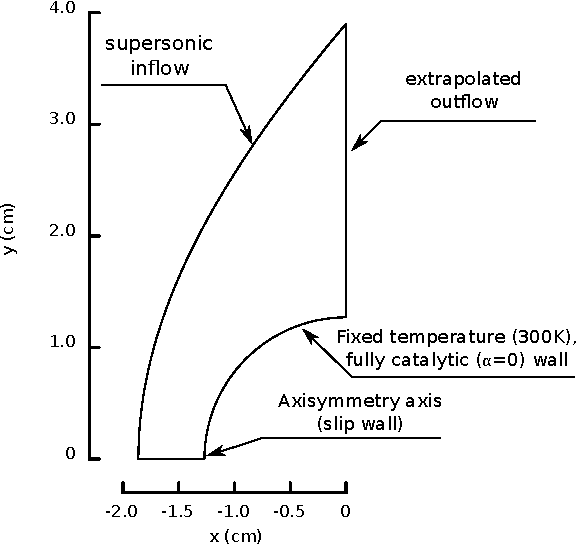
\includegraphics[width=0.49\linewidth]{../2D/Rutowski-hemisphere/figures/domain.pdf}
  \label{fig:rutowskiDomain}
 }
 \subfloat[Computation grid] {
  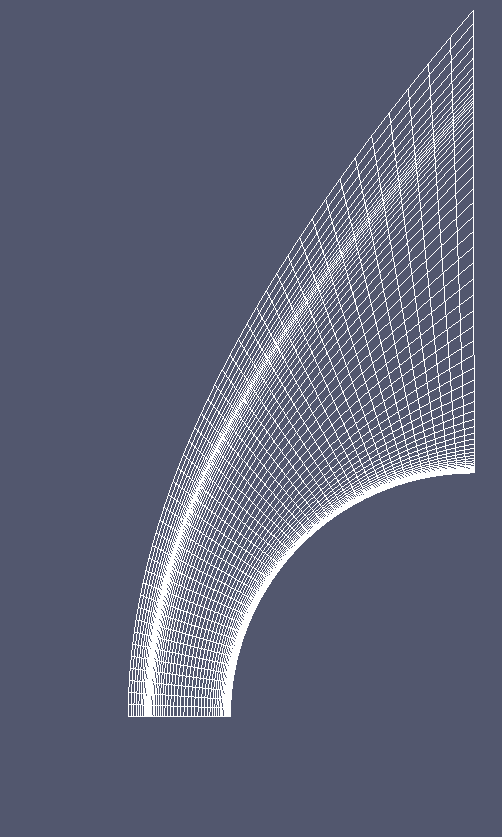
\includegraphics[width=0.28\linewidth]{../2D/Rutowski-hemisphere/figures/grid.png}
  \label{fig:rutowskiGrid}
 }
 \caption{Computational domain and grid for Navier--Stokes simulations of the Rutowski and Bershader~\cite{RB64} experiments.}
\end{figure}

\subsubsection{Thermodynamics}

The argon plasma is modelled via the consideration of three species (Ar, Ar$^+$ and e$^-$) and two temperatures (a heavy particle translation temperature, $T$, and a combined free electron and bound electronic temperature, $T_e$).
This allows the nonequilibrium between heavy-particle and free-electron translation to be captured whilst acknowledging the efficiency of bound electronic excitation via free electron impact.
The electronic energy of the heavy particle species are calculated assuming Boltzmann distribution of the electronic state populations.
The electronic level structure of Ar and Ar$^+$ are represented with 8 and 13 grouped levels, respectively, using the energy level from NIST ASD~\cite{NIST_ASD}. 

\subsubsection{Viscous transport}

Viscosity and thermal conductivity are calculated via the Gupta-Yos model~\cite{GYT+90}.
The collision integrals are compiled from  Wright \textit{et al.}~\cite{WBP+2005}, Levin \textit{et al.}~\cite{LW2005} and Mason~\textit{et al.}~\cite{Mas67}.
Species mass diffusion is not considered.

\subsubsection{Chemical reactions}

Three chemical reactions are considered:

\begin{eqnarray}
 \text{Ar + Ar} &\leftrightharpoons& \text{Ar$^+$ + e$^-$ + Ar} \label{eq:HPII} \\
 \text{Ar + Ar$^+$} &\leftrightharpoons& \text{Ar$^+$ + e$^-$ + Ar$^+$} \label{eq:HPII+} \\
 \text{Ar + e$^-$} &\leftrightharpoons& \text{Ar$^+$ + e$^-$ + e$^-$}  \label{eq:EII} \\
 \end{eqnarray}
 
 \noindent where photoionization has been omitted based on its relatively minor contribution for other high enthalpy conditions~\cite{Cam91} .
 The reaction rates are determined via fitting an Arrhenius equaion to the two-stage model proposed by Petschek \textit{et al.}~\cite{PB57}:
 
 \begin{equation}
 k_{f,M}(T_M) = S_{Ar-M}^* \sqrt{ \frac{32}{\pi} \left ( \frac{m_{Ar} + m_M}{m_{Ar} m_M} \right ) } \cdot \left ( k_B T_M \right )^\frac{3}{2} \left ( \frac{\Theta_{1}}{2T_M} + 1 \right ) \text{exp} \left ( - \frac{\Theta_{1}}{T_M} \right )
\end{equation}

\noindent where $S_{Ar-M}^*$ is the first excitation collision cross-section for colliding particle $M$, $T_M$ is the translational temperature of the colliding particle and $\Theta_1$ is the characteristic temperature of the first excited state of argon (134,800\,K).
Glass \textit{et al.}~\cite{GL78} found good agreement with shock tube electron density profiles using $S_{Ar-Ar}^* = 1.0 \times 10^{-19}$ and $S_{Ar-e^-}^* = 4.9 \times 10^{-18}$\,cm$^2$/eV; these cross-section are therefore used in the present work.
 
\subsubsection{Thermal energy exchange}

Translational energy exchange due to elastic collisions between free electrons and heavy particles is calculated via the model proposed by Appleton \textit{et al.}~\cite{appleton_1964}.
The e$^{-}$--Ar effective elastic collision cross-section are taken from Jaffrin~\cite{Jaf65}.

\subsubsection{Radiation transport}

A photon Monte--Carlo model is implemented to numerically solve for the both the radiative divergence throughout the flowfield ($\nabla \cdot \vec{q}_\text{rad}$), and the radiative heating incident on solid surfaces ($q_\text{rad}$).
The basis of photon Monte--Carlo models~\cite{HP64,Mod92,WM2007} is the modelling of radiation transport by a collection of photon bundles with statistically determined properties.
For the present simulations, a maximum of 32768 photons-per-cell are emitted, and their absorption throughout the flowfield is modelled via the partitioned energy model~\cite{MP77}.
See \textsection~4.5 of the Eilmer3 theory book (\url{http://cfcfd.mechmining.uq.edu.au/pdf/eilmer3-theory-book.pdf}) for a detailed description of the model.

\subsubsection{Radiation spectra}

The radiation spectra of the argon plasma are calculated via the Photaura model (see \url{http://cfcfd.mechmining.uq.edu.au/pdf/photaura-users-guide.pdf}).
Three radiation mechanisms are considered:

\begin{enumerate}
 \item Bound-bound line radiation
 \item Photoionization continuum radiation
 \item Bremsstrahlung continuum radiation
\end{enumerate}

425 individual Ar lines and 307 individual Ar$^+$ lines from the NIST ASD~\cite{NIST_ASD} are considered, and  photoionization cross-sections are obtained from TOPBase~\cite{TOPbase}.
The experimentally measured Stark widths for 48 Ar lines collated by Griem~\cite{Griem74} are implemented, with the remaining lines using the empirical fit suggested by Park~\cite{Park82}.
The upper and lower state populations for the Ar atom are determined via application of a collisional-radiative model in the QSS limit~\cite{park_1990}.
The spectral grid is uniformally distributed in wavenumber space in the range $1000 \leq \eta \leq 150000$~$^{1/\text{cm}}$, with a resolution of 1 point / 10~$^{1/\text{cm}}$.

\subsection{Results}

Temperature solutions from Eilmer3 simulation of the Rutowski hemisphere with radiation-flowfield coupling are presented in Figure~\ref{fig:rutowskiTemperature}.
Immediately behind the shock there is a region of thermal nonequilibrium, with the electron temperature being significantly lower than the heavy particle temperature.
Both temperatures radidly drop towards the 300K wall temperature near the model surface.

\begin{figure}
 \centering
 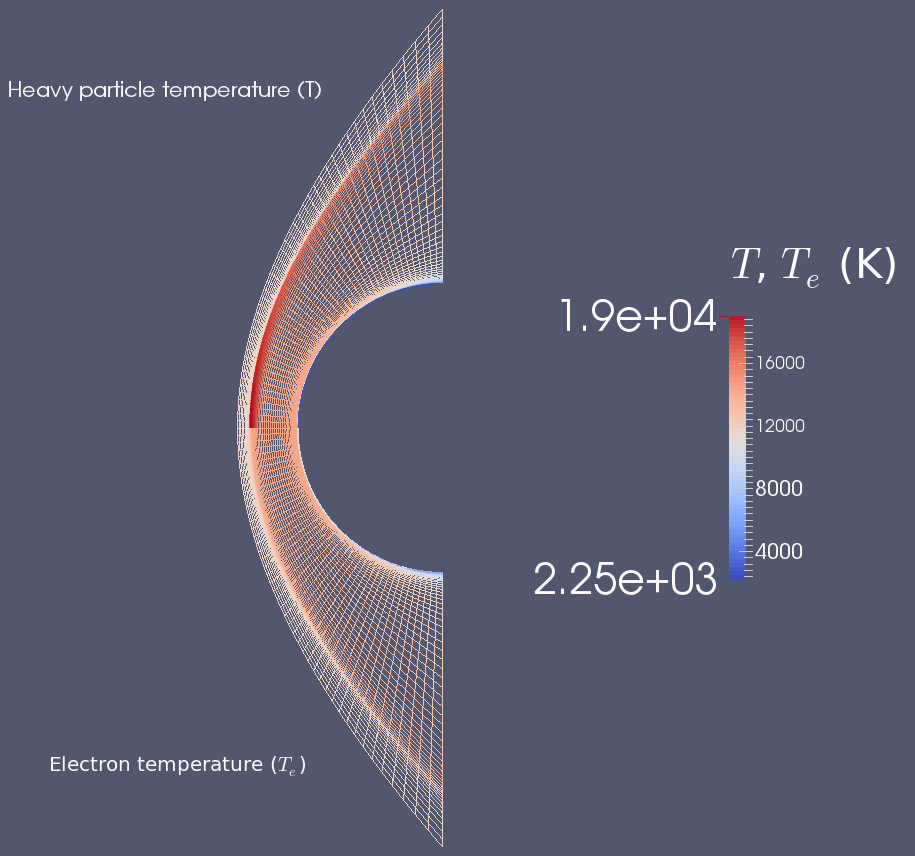
\includegraphics[width=0.7\linewidth]{../2D/Rutowski-hemisphere/figures/temperature.png}
 \caption{Temperature solutions from Eilmer3 simulation of the Rutowski hemisphere with radiation-flowfield coupling.}
 \label{fig:rutowskiTemperature}
\end{figure}

The radiation solution is presented in Figure~\ref{fig:rutowskiRadiation}.
The hot shock layer is a net emitter of radiation (blue), whilst the cool and dense boundary layer is a net absorbed of radiation (red).

\begin{figure}
 \centering
  \subfloat[Full computational domain] {
  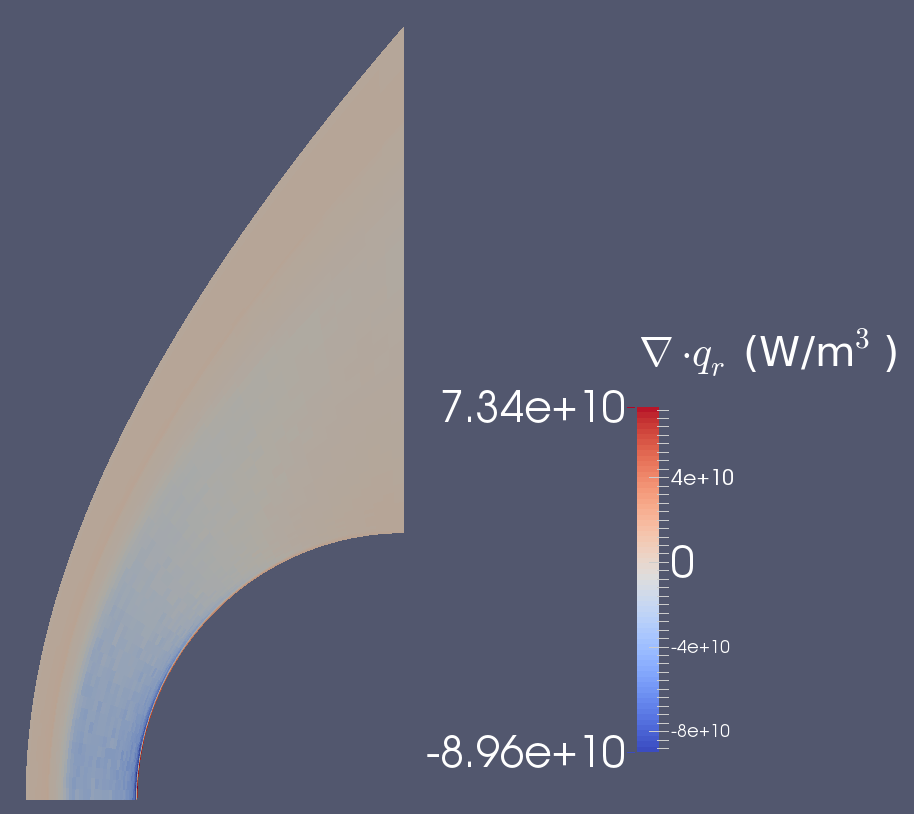
\includegraphics[width=0.49\linewidth]{../2D/Rutowski-hemisphere/figures/radiation.png}
 }
  \subfloat[Stagnation point detail] {
  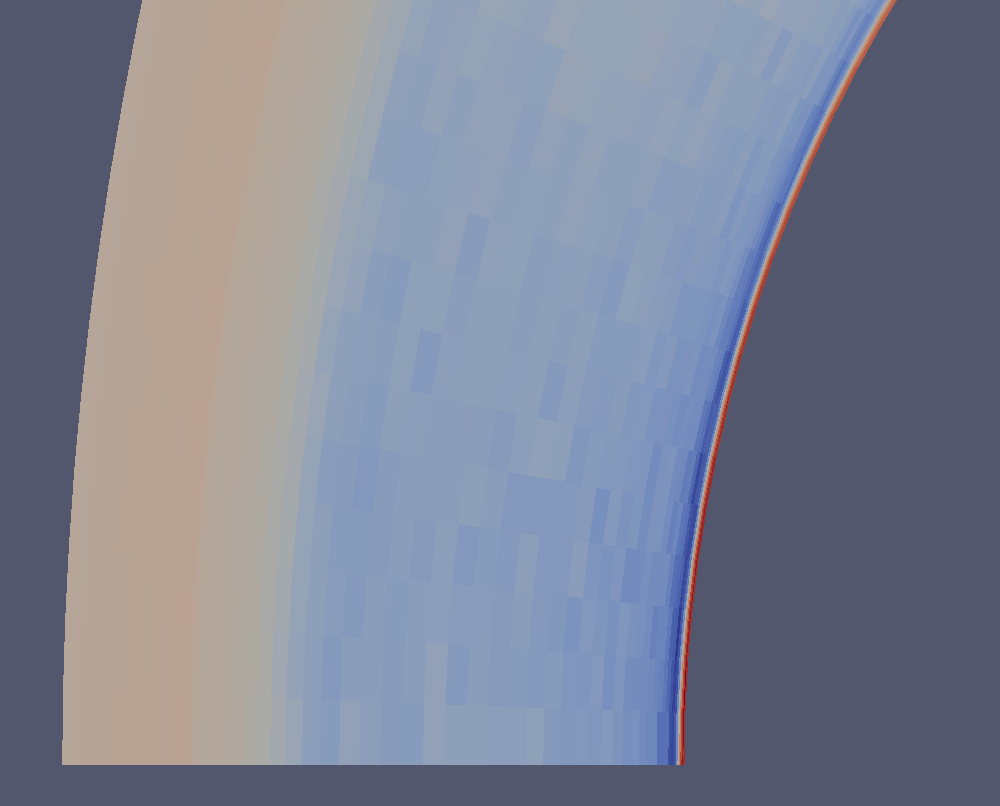
\includegraphics[width=0.49\linewidth]{../2D/Rutowski-hemisphere/figures/radiationDetail.png}
 }
 \caption{Radiation solution from Eilmer3 simulation of the Rutowski hemisphere with radiation-flowfield coupling.}
  \label{fig:rutowskiRadiation}
\end{figure}

The computed surface radiative heating profiles are compared with the experiment measurements in Figure~\ref{fig:rutowskiResults}.
The computed result at the stagnation point in the spectral range $67 \leq \lambda \leq 10000$\,nm of approximately 5.1~kW/cm$^2$ is in agreement with the blackened guage data to within the measurement uncertainty bounds.
The computed result for the supposed range of sensitivity for the radiometer ($180 \leq \lambda \leq 6000$\,nm), however, is slightly lower than the measured data.
A finer spectral grid may improve the agreement with experiment by allowing the peaks of the atomic lines to be better resolved.

\begin{figure}
 \centering
 \caption{Radiative heating on the hemisphere surface: Eilmer3 for $67 \leq \lambda \leq 10000$\,nm (\ref{plt:rutowskiE3All}), Eilmer3 for $180 \leq \lambda \leq 6000$\,nm (\ref{plt:rutowskiE3Limited}), experiment with blackened gauge (\ref{plt:rutowskiExpBlackened}) and experiment with adjust gauge (\ref{plt:rutowskiExpAdjusted})} 
 \begin{tikzpicture}[baseline]
 % \selectcolormodel{gray}
  \begin{axis}[grid=major,
                           xlabel={$\theta$ ($^\circ$)},
                           ylabel={$q_\text{rad}$ (kW/cm$^2$)},
                           width=0.8\textwidth,
                           height=0.6\textwidth,
                         ]
  \addplot[thick,dashed,color=black,no marks]
                    table[x=theta,y=qrad]
                   {../2D/Rutowski-hemisphere/Ms_12.70/calculated/qrad-all.txt};
  \label{plt:rutowskiE3All}
    \addplot[thick,color=black,no marks]
                    table[x=theta,y=qrad]
                   {../2D/Rutowski-hemisphere/Ms_12.70/calculated/qrad-limited.txt};
  \label{plt:rutowskiE3Limited}
  \addplot+[only marks,mark size=4,color=black,fill=black,mark=*,error bars/y dir=both,error bars/y fixed relative=0.162]
                       table[x=theta,y=qrad]
                      {../2D/Rutowski-hemisphere/Ms_12.70/measured/blackened_radiometer.txt};
  \label{plt:rutowskiExpBlackened}
  \addplot+[only marks,mark size=4,color=black,mark=o,error bars/y dir=both,error bars/y fixed relative=0.162]
                       table[x=theta,y=qrad]
                      {../2D/Rutowski-hemisphere/Ms_12.70/measured/adjusted_radiometer.txt};
  \label{plt:rutowskiExpAdjusted}	
  \end{axis}
  \end{tikzpicture}
 \label{fig:rutowskiResults}
\end{figure}

\subsection{Run script (.sh)}

\topbar
\lstinputlisting[language={}]{../2D/Rutowski-hemisphere/Ms_12.70/run.sh}
\bottombar

\subsection{Eilmer3 input scripts (.py)}

\subsubsection{Part 1 -- inviscid flow}

\topbar
\lstinputlisting[language={}]{../2D/Rutowski-hemisphere/Ms_12.70/part1-inviscid/hemisphere.py}
\bottombar

\subsubsection{Part 2 -- viscous flow}

\topbar
\lstinputlisting[language={}]{../2D/Rutowski-hemisphere/Ms_12.70/part2-viscous/hemisphere.py}
\bottombar

\subsubsection{Part 3 -- viscous flow with radiation coupling}

\topbar
\lstinputlisting[language={}]{../2D/Rutowski-hemisphere/Ms_12.70/part3-viscous-with-radiation/hemisphere.py}
\bottombar

\subsection{Chemical reaction script (.lua)}

\topbar
\lstinputlisting[language={}]{../2D/Rutowski-hemisphere/kinetic-models/Ar-2T-chemical-reactions.lua}
\bottombar

\subsection{Thermal energy exchange script (.lua)}

\topbar
\lstinputlisting[language={}]{../2D/Rutowski-hemisphere/kinetic-models/Ar-2T-energy-exchange.lua}
\bottombar

\subsection{Radiation model (for flowfield coupling) script (.py)}

\topbar
\lstinputlisting[language={}]{../2D/Rutowski-hemisphere/Ms_12.70/part3-viscous-with-radiation/Ar-nonequilibrium-radiation.py}
\bottombar

\subsection{Radiation model (for experiment comparison) script (.py)}

\topbar
\lstinputlisting[language={}]{../2D/Rutowski-hemisphere/Ms_12.70/part3-viscous-with-radiation/Ar-nonequilibrium-radiation-180to6000nm.py}
\bottombar

% \subsection{Tcl run script}
% \topbar
% \lstinputlisting[language={}]{../2D/Rutowski-hemisphere/Ms_12.70/Rutowski-long.test}
% \bottombar

\subsection{Radiation error checking script (.py)}
\topbar
\lstinputlisting[language={}]{../2D/Rutowski-hemisphere/Ms_12.70/compute_qrad_error.py}
\bottombar

\subsection{Notes}

\begin{itemize}
 \item The radiation-flowfield coupling is relatively weak for this case, and therefore the flowfield solution with and without radiation are relatively similar.
For cases where radiation-flowfield coupling is stronger, difficulties may arise when the scaling of the radiation source term is turned on.
 \item The radiation portion of this simulation can be run in parallel on a shared memory computer.  See \url{http://cfcfd.mechmining.uq.edu.au/eilmer3.html#building-and-running-the-radiation-transport-solver} for intructions on how to compile \texttt{e3rad.exe} for parallel computations.
\end{itemize}